\subsection{بخش چ}
این بخش به بررسی تغیر زاویه $\psi$ هدف پرداخته است. فاصله ازدست‌دهی در جدول زیر آمده است.

\begin{table}[H]
	\caption{فاصله ازدست‌دهی در شرایط اولیه مختلف هدف }
	\centering
	\begin{tabular}{cc}
		\hline
		\lr{Miss Distance (m)} &  $\psi$ \\
		\hline
		$0.6022$ & \lr{\ang{180}}\\
		$5212.3835$  & \lr{\ang{0}} \\ 
		\hline
	\end{tabular}
\end{table}
نمودار نتایج در ادامه آورده شده است.
\begin{figure}[H]
	\centering
	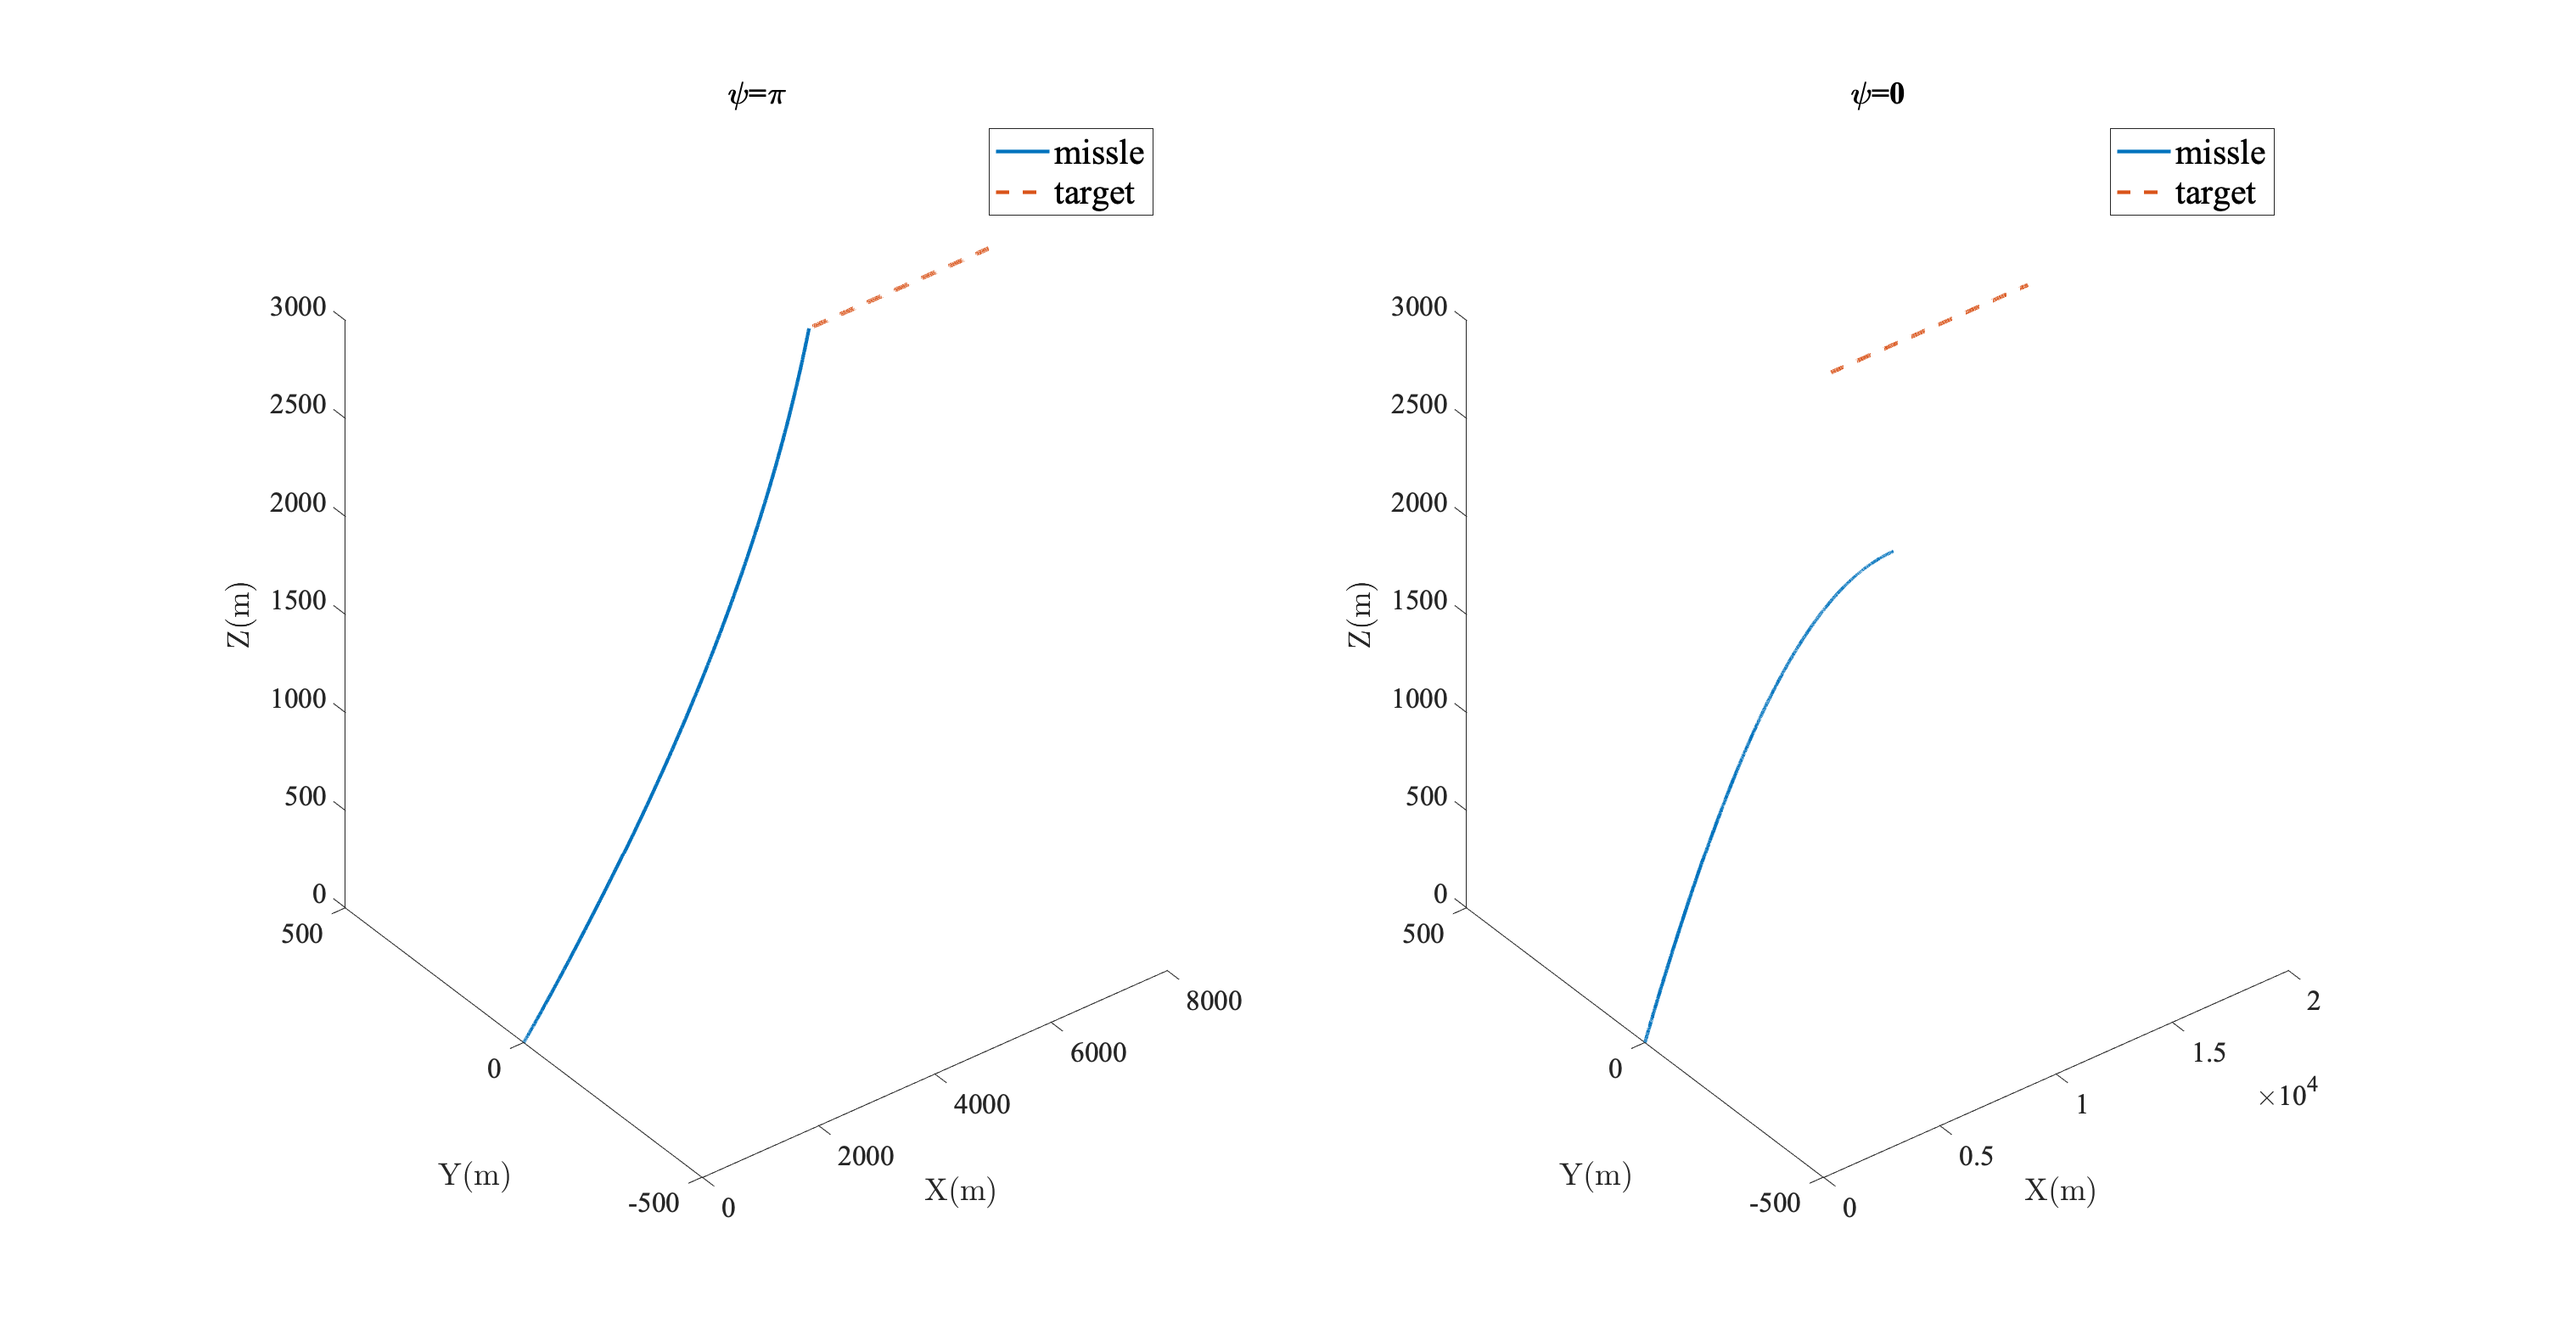
\includegraphics[width=\linewidth]{../Figure/g/3DoF_missle_vs_target_state}
	\caption{مقایسه موقعیت موشک و هدف به صورت سه بعدی در دو نمودار با شرایط اولیه مختلف هدف در هدایت خط دید پایه همراه با مشتق‌گیر}
\end{figure}

\begin{figure}[H]
	\centering
	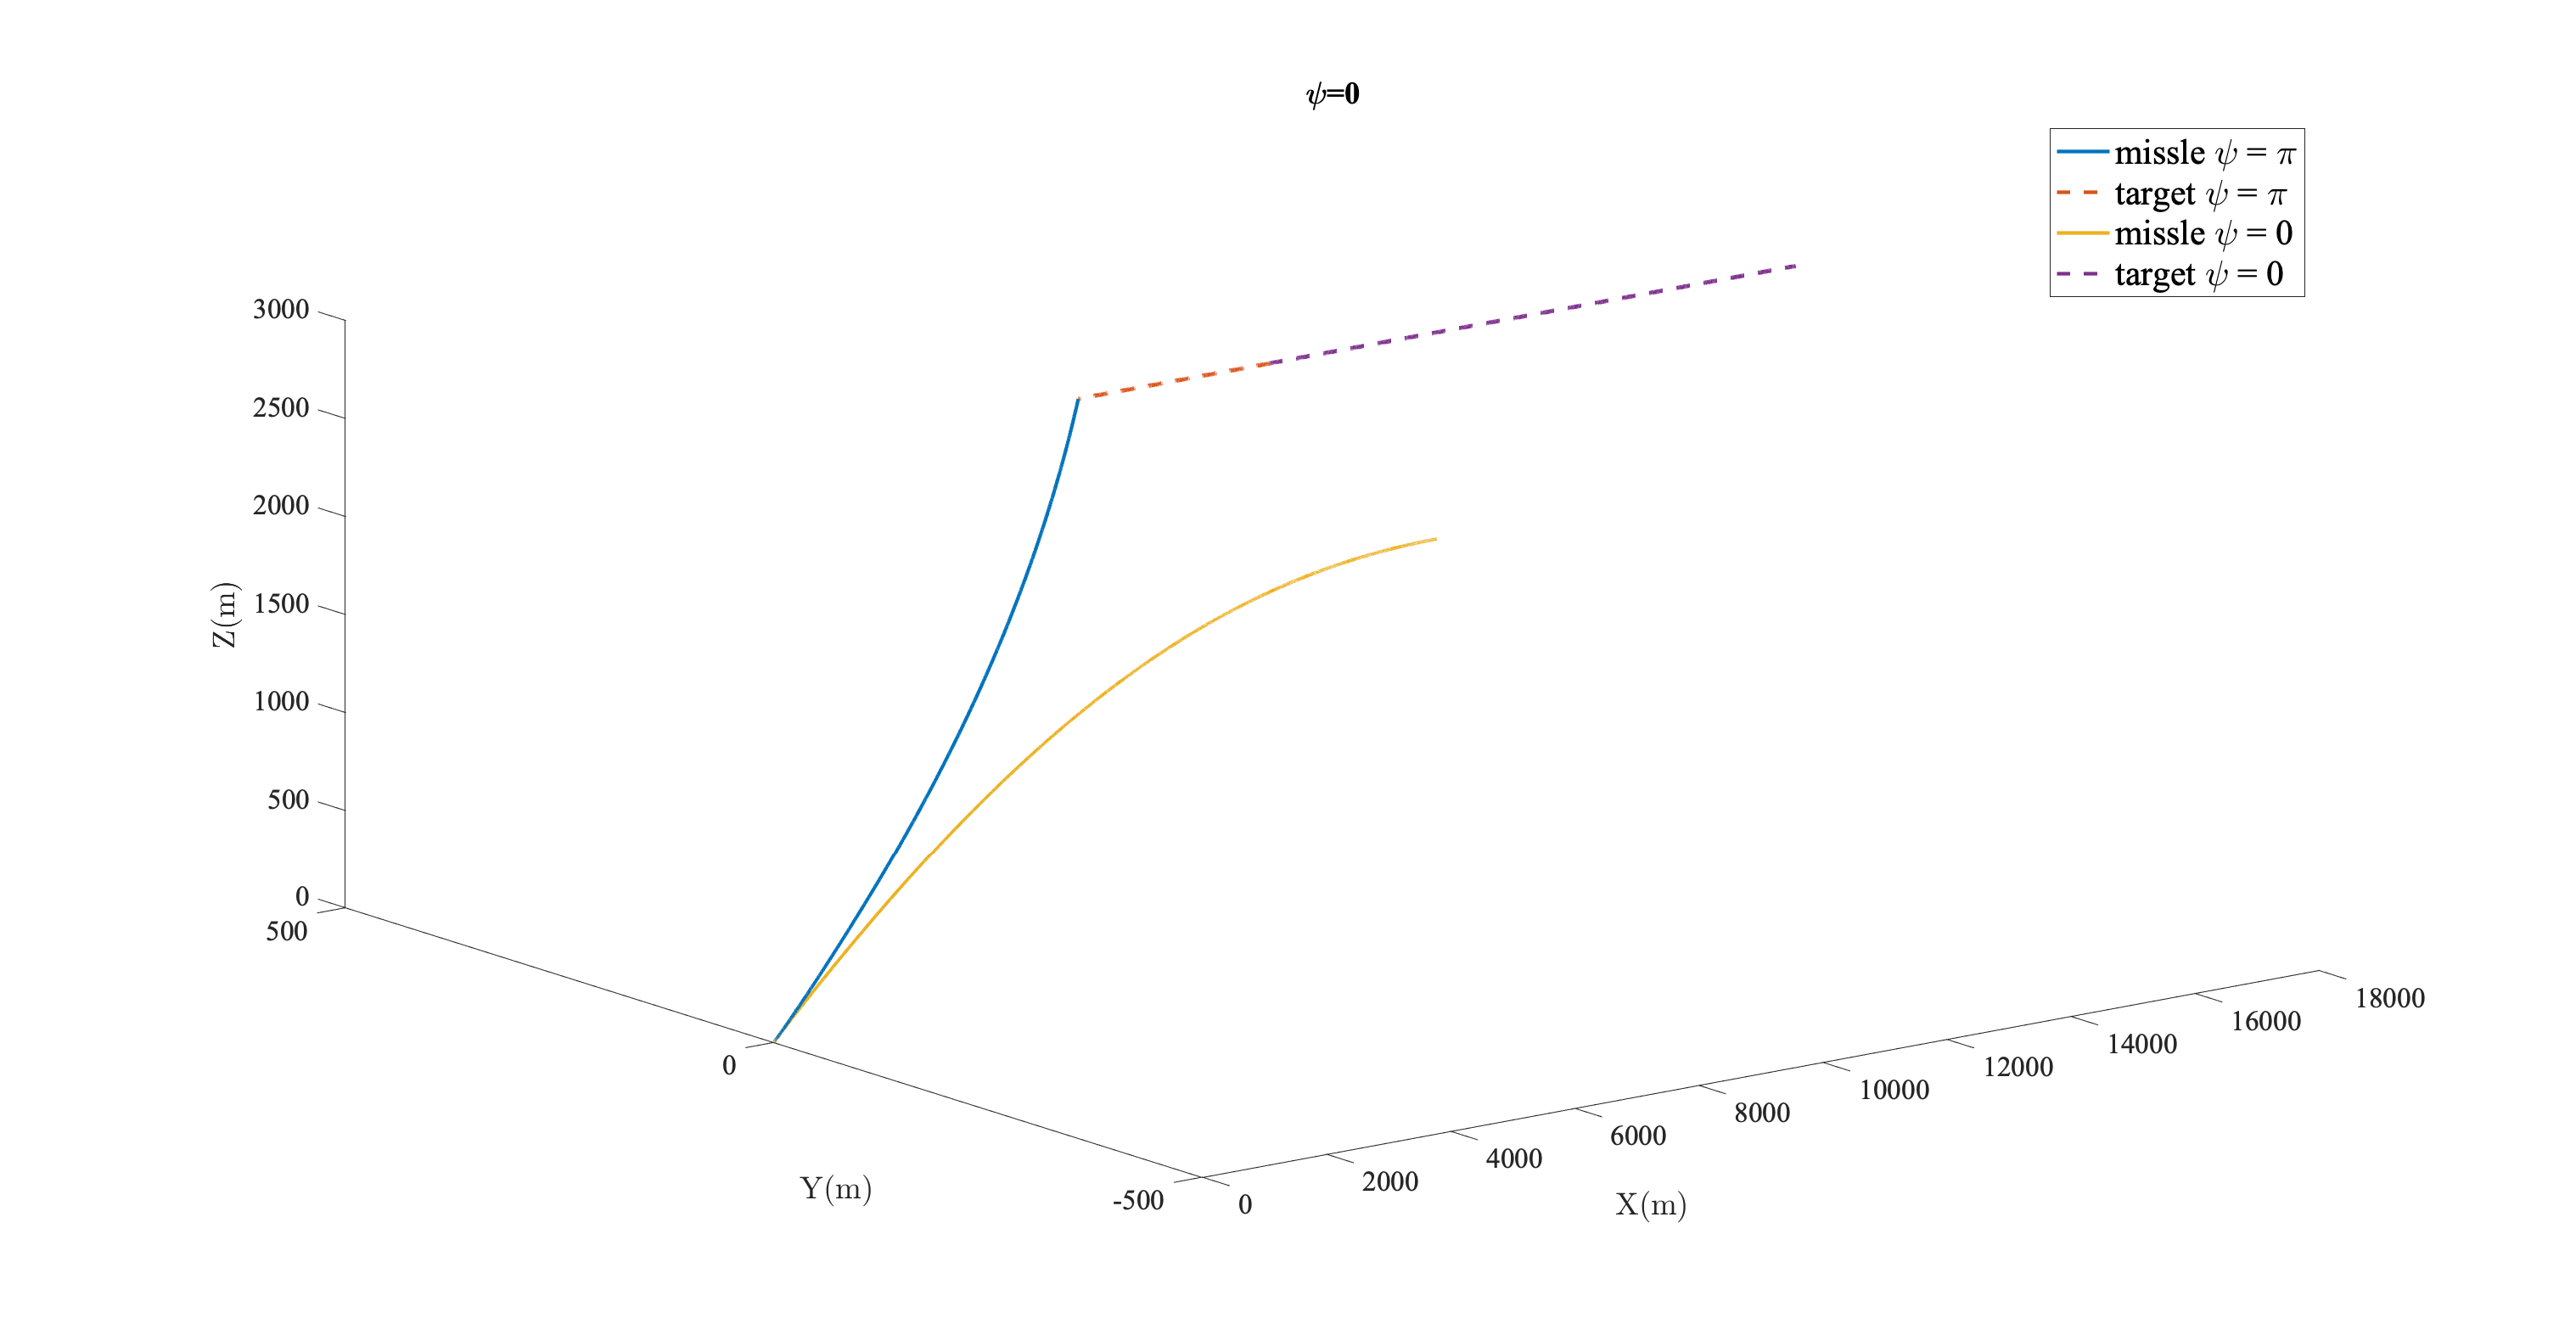
\includegraphics[width=\linewidth]{../Figure/g/3DoF_missle_vs_target_state_all_in}
	\caption{مقایسه موقعیت موشک و هدف به صورت سه بعدی در یک نمودار با شرایط اولیه مختلف هدف در هدایت خط دید پایه همراه با مشتق‌گیر}
\end{figure}

\begin{figure}[H]
	\centering
	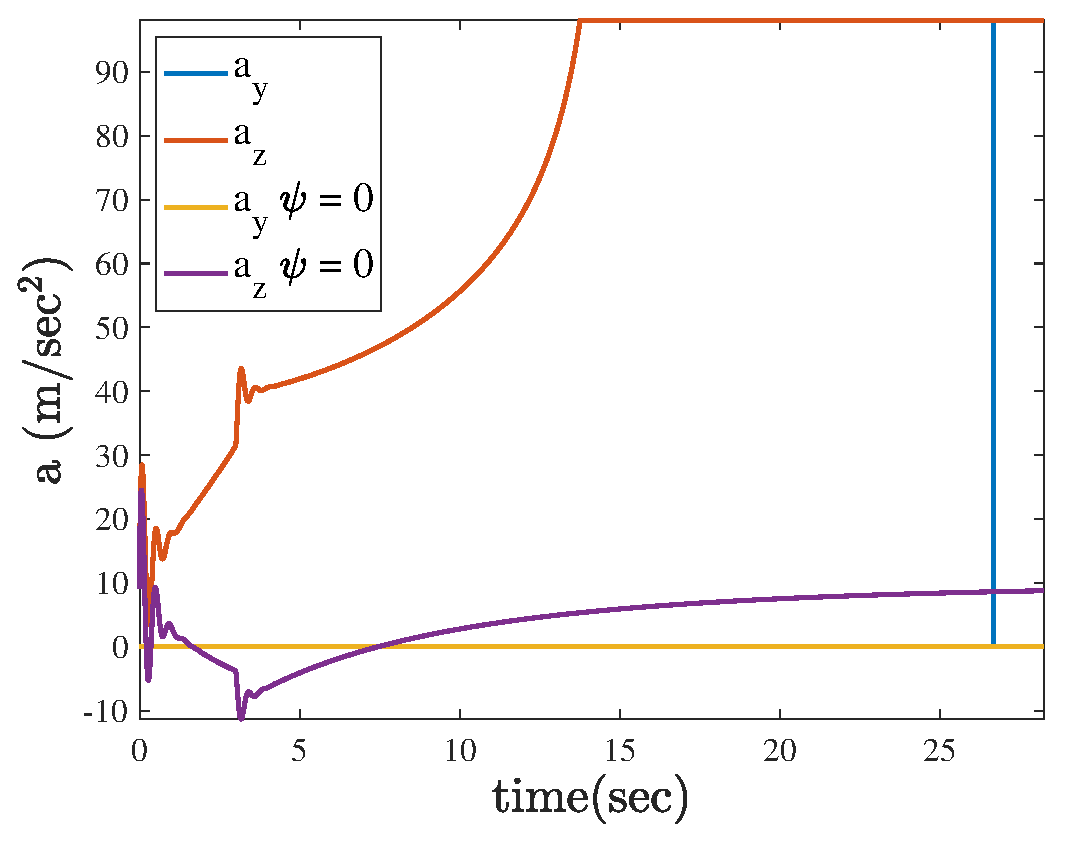
\includegraphics[width=.75\linewidth]{../Figure/g/command}
	\caption{مقایسه فرمان موشک با شرایط اولیه مختلف هدف در هدایت خط دید پایه همراه با مشتق‌گیر}
\end{figure}

\begin{figure}[H]
	\centering
	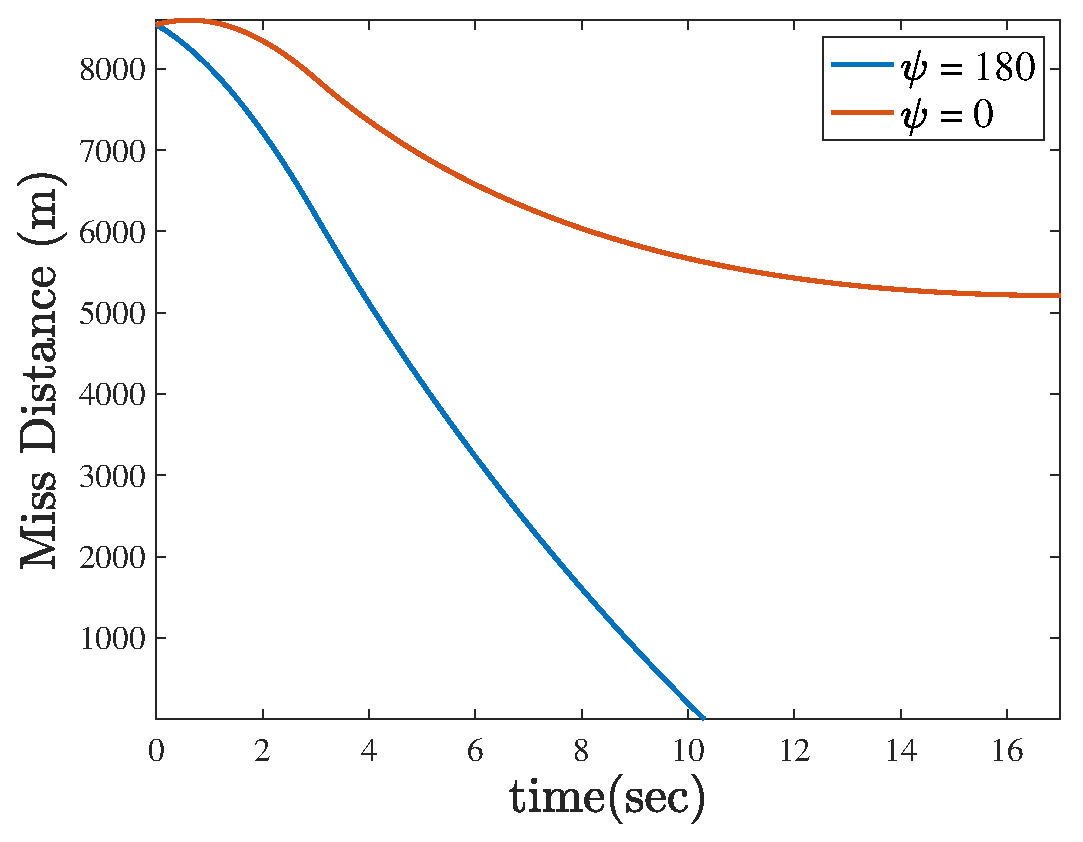
\includegraphics[width=.75\linewidth]{../Figure/g/miss_distance}
	\caption{مقایسه فاصله ازدست‌دهی موشک با شرایط اولیه مختلف هدف در هدایت خط دید پایه همراه با مشتق‌گیر}
\end{figure}

در ادامه با استفاده از الگوریتم \lr{Greedy} کمینه سرعت برای فاصله ازدست‌دهی کمتر از ۱۵ متر بدست آمد. با توجه به اینکه در حالت اول عمکرد بهتری دارد پس اگر حالت دو ارضا شود، حالت یک هم حتما ارضا می‌شود

\begin{table}[H]
	\caption{فاصله ازدست‌دهی در شرایط اولیه مختلف هدف }
	\centering
	\begin{tabular}{ccc}
		\hline
		\lr{Miss Distance (m)} &  $\psi$ & \lr{V (m/sec)} \\
		\hline
		$0.6022$ & \lr{\ang{180}} & \lr{300} \\
		$5212.3835$  & \lr{\ang{0}} & \lr{300} \\
		$0.3293$ & \lr{\ang{180}} &\lr{ 106.9} \\
		$14.4173 $  & \lr{\ang{0}} & \lr{106.9} \\
		\hline
	\end{tabular}
\end{table}
نمودار نتایج در ادامه آورده شده است.

\begin{figure}[H]
	\centering
	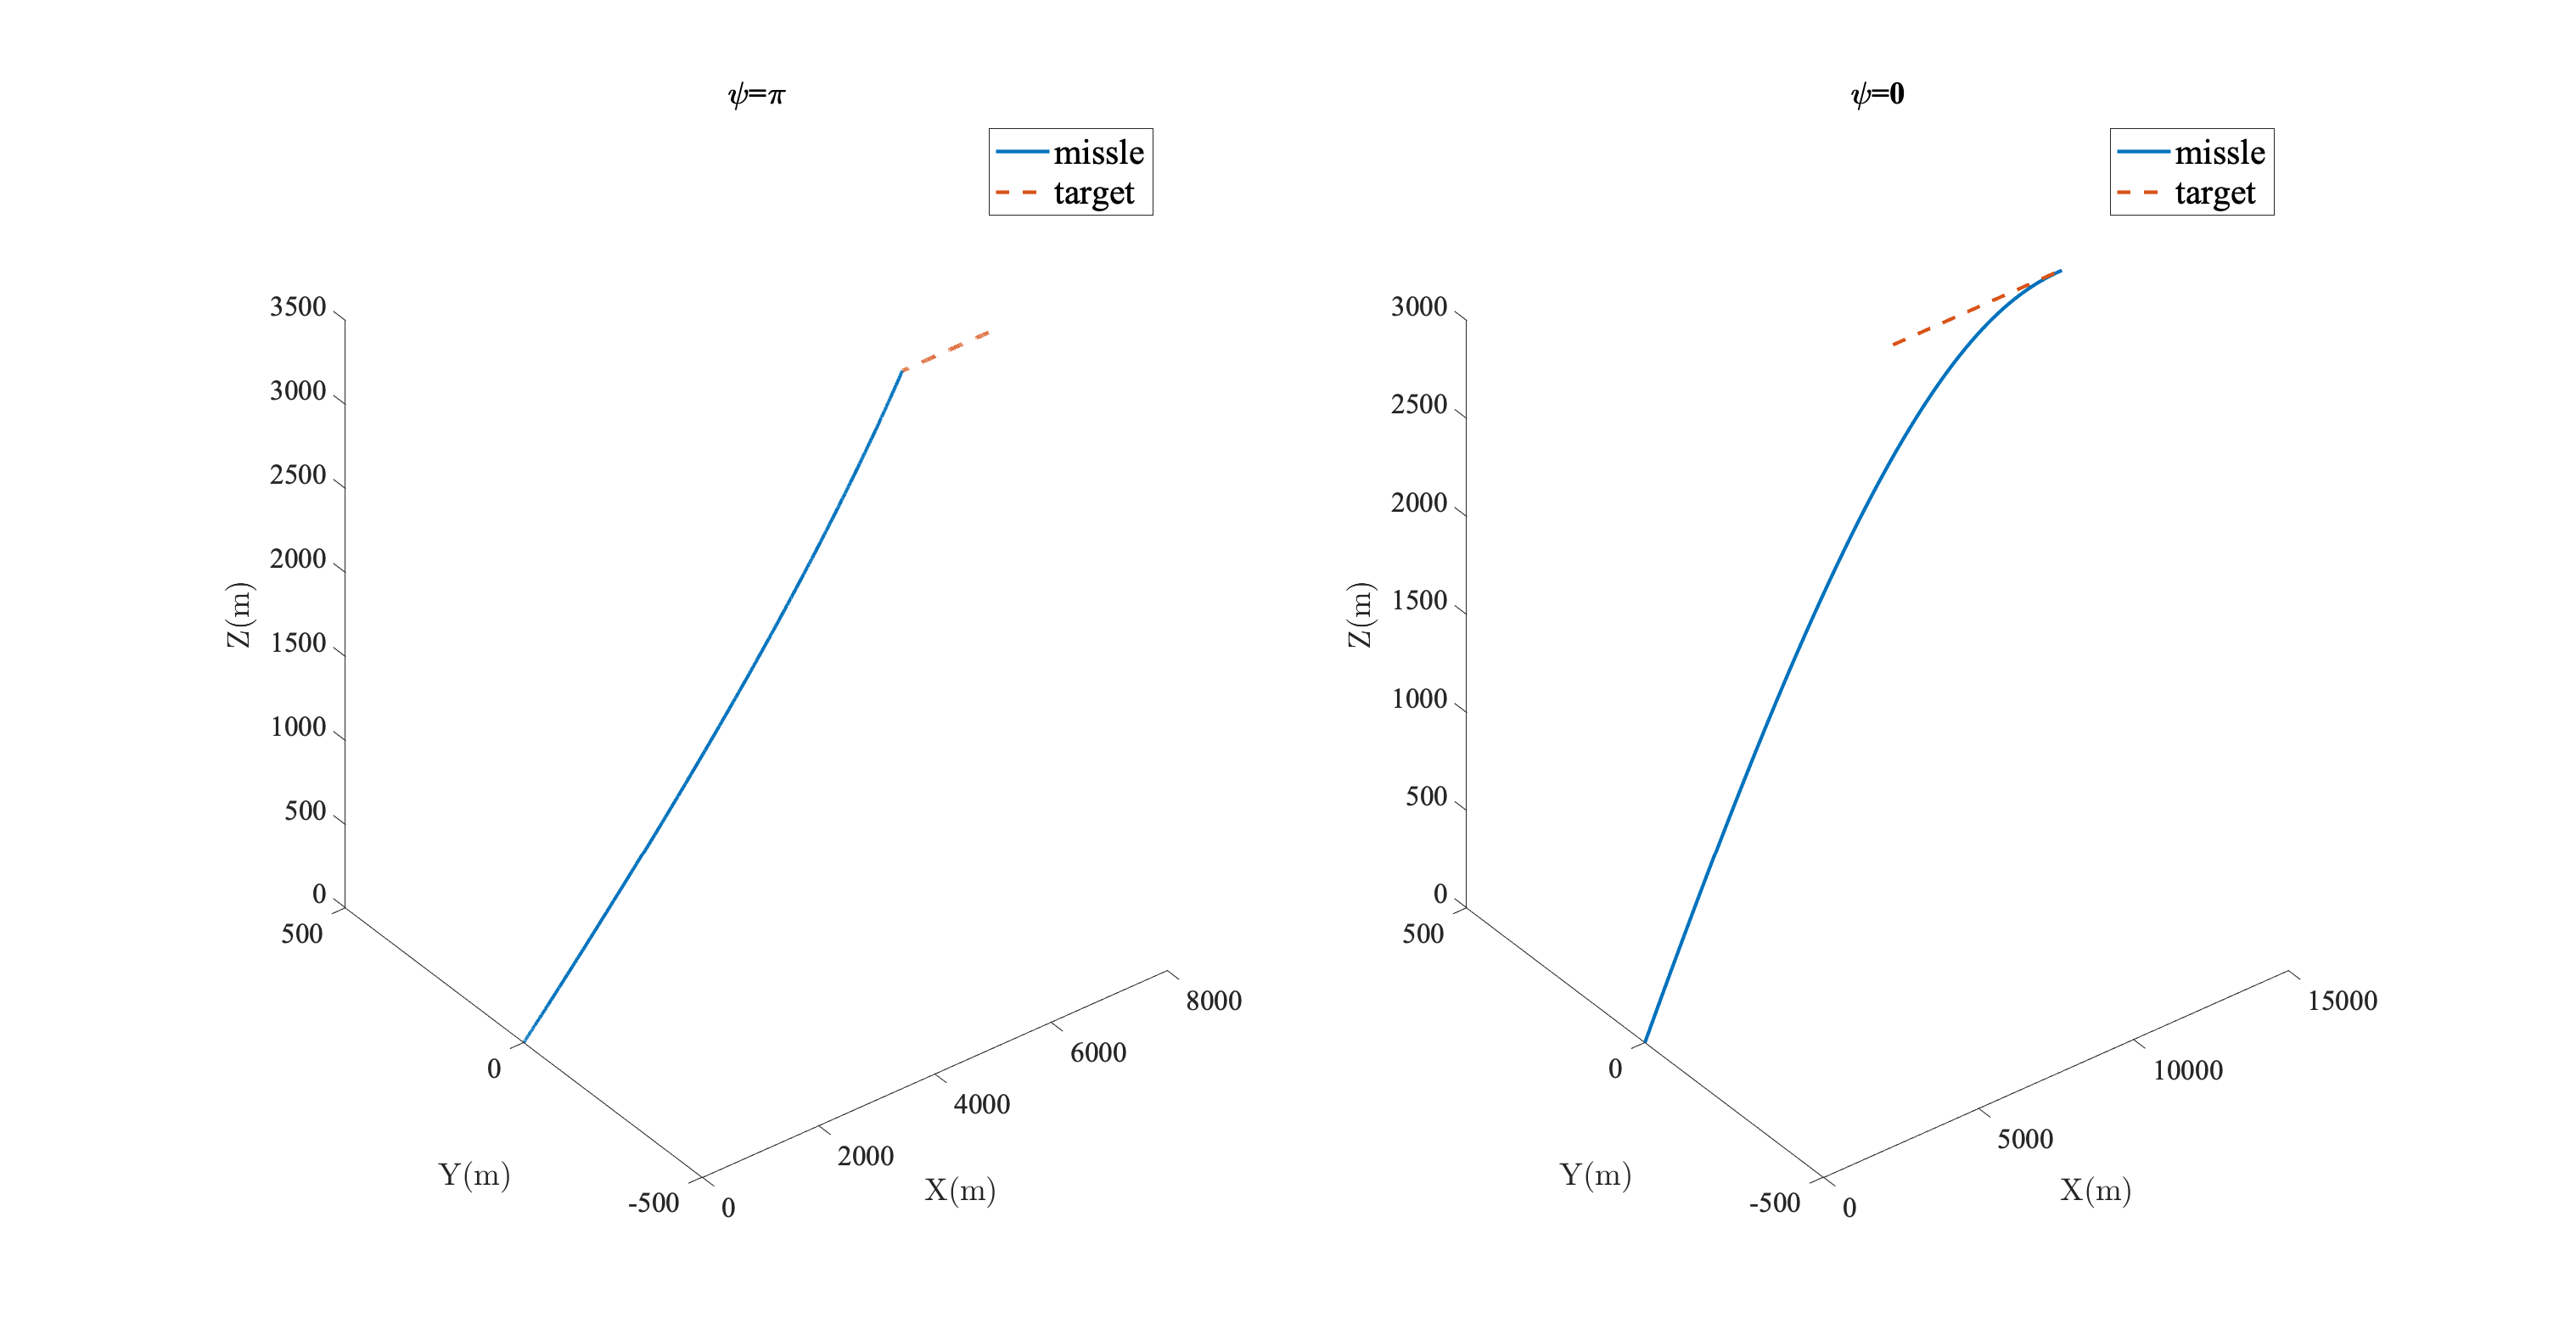
\includegraphics[width=\linewidth]{../Figure/g/3DoF_missle_vs_target_state_low_v}
	\caption{مقایسه موقعیت موشک و هدف به صورت سه بعدی در دو نمودار با شرایط اولیه مختلف هدف و کمینه سرعت اولیه جهت فاصله ازدست‌دهی کمتر از ۱۵ متر در هدایت خط دید پایه همراه با مشتق‌گیر}
\end{figure}

\begin{figure}[H]
	\centering
	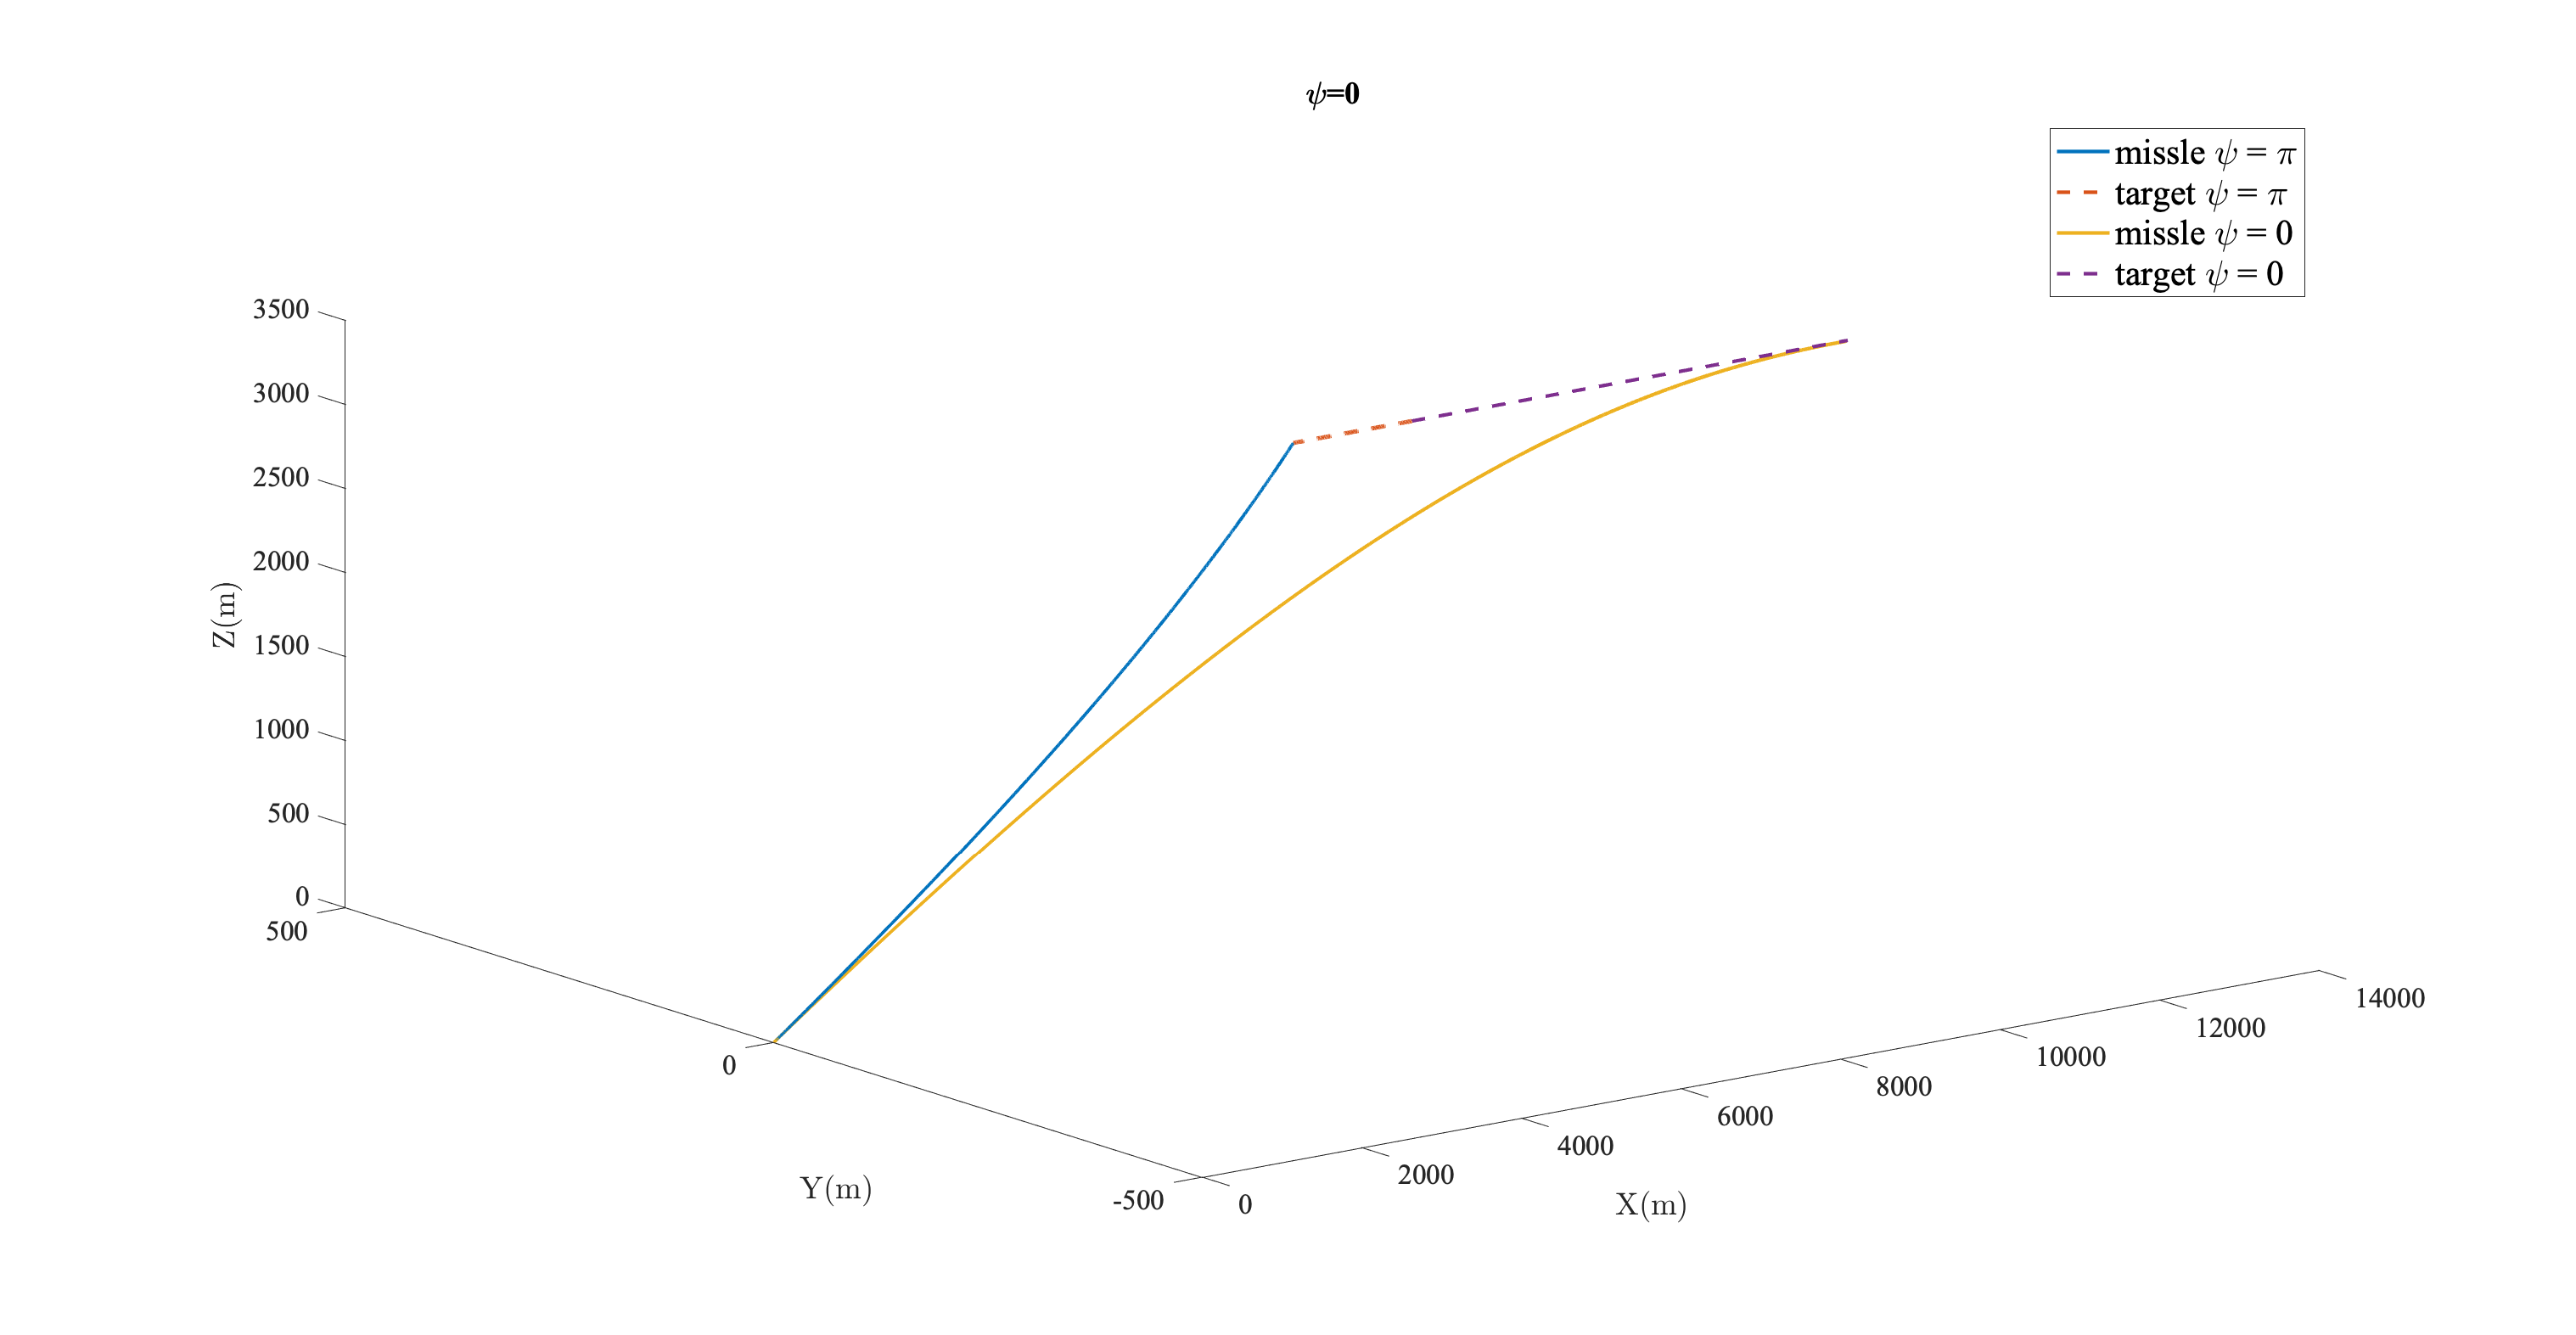
\includegraphics[width=\linewidth]{../Figure/g/3DoF_missle_vs_target_state_all_in_low_v}
	\caption{مقایسه موقعیت موشک و هدف به صورت سه بعدی در یک نمودار با شرایط اولیه مختلف هدف و کمینه سرعت اولیه جهت فاصله ازدست‌دهی کمتر از ۱۵ متر در هدایت خط دید پایه همراه با مشتق‌گیر}
\end{figure}



